\section{Theoretical Foundations}
\label{sec:Theoretical_Foundations}
In this experiment the speed of sound in various solids and liquids was determined. This section summarizes the theory and formulas necessary to understand the following experiments on ultrasound in section \ref{sec:Evaluation}.

%-------------------------------------------------------------------------------------------
\subsection{Wave Propagation}
\label{subsec:Wave_Propagation}
Wave propagation is the way in which waves travel. It can be distinguished between transverse waves and longitudinal waves. These waveforms are defined as follows:

\textbf{Transverse wave:} The displacement of the medium the wave travels through is perpendicular to the direction in which the wave propagates. Figure \ref{fig:transverse} shows a graphical representation of this sinusoidal waveform in a rope \cite{waves}.

\begin{figure}[H]
	\centering
	\includegraphics[scale=0.4]{transverse}
	\caption{Representation of a periodic transverse sinusoidal wave in a rope. The up and down motion of the rope is perpendicular to the direction in which the wave propagates. This leads to each particle of the rope moving up and down \cite{waves}. - partially modified}
	\label{fig:transverse}
\end{figure}

\textbf{Longitudinal wave:} The displacement of the medium the wave travels through is parallel to the direction in which the wave propagates. Sound waves in air behave like this. The air molecules oscillate back and forth and their energy is propagated in the same direction as their motion. Figure \ref{fig:longitudinal} shows a graphical representation of this waveform in a mechanical spring \cite{waves}.

\begin{figure}[H]
	\centering
	\includegraphics[scale=0.45]{longitudinal}
	\caption{Representation of a longitudinal wave in a mechanical spring. The elastic deflection (compression and extension) of the spring is parallel to the direction in which the wave propagates. This produces areas of increased and decreased pressure \cite{waves}.}
	\label{fig:longitudinal}
\end{figure}

\newpage
%-------------------------------------------------------------------------------------------
\subsection{Reflection and Refraction}
\label{subsec:Reflection_and_Refraction}
Similar to optics, reflection and refraction also occur when sound waves hit the boundary between two different media. Contrary to optics, the refraction index is not the important quantity. The phase velocity leads to refraction and the impedance leads to reflection. It can be distinguished between a vertical and an oblique angle of incidence. The following two sections explain this in more detail \cite{ultrasound}.

%-------------------------------------------------------------------------------------------
\subsubsection{Vertical Angle of Incidence}
\label{subsubsec:Vertical_Angle_of_Incidence}
A sound wave with the pressure $\hat{p}_e$ and velocity $v_e$ that travels trough a medium with the impedance $Z_1$ hits a boundary between two media with a vertical angle of incidence. This results in a different ratio between the pressure $\hat{p}_t$ and velocity $v_t$ in the medium with the impedance $Z_2$. At the same time the pressure and the velocity have to be equal at the boundary between the two media. This leads to a third reflected partial wave. Figure \ref{fig:vertical_angle_of_incidence} shows the just described phenomenon \cite{ultrasound}.

\begin{figure}[H]
	\centering
	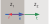
\includegraphics[scale=1.5]{vertical_angle_of_incidence}
	\caption{Representation of a sound wave $e$ in blue that hits a boundary between the two media with the impedances $Z_1$ and $Z_2$. The transmitted wave $t$ is shown in green and the reflected partial wave $r$ is shown in red \cite{ultrasound}. - partially modified}
	\label{fig:vertical_angle_of_incidence}
\end{figure}

The calculation of the amplitude reflection coefficient $r$ is shown in equation \ref{eq:vertical_reflection} and the amplitude transmission coefficient $t$ is shown in equation \ref{eq:vertical_transmission}. They can be derived by utilizing the continuity conditions that are valid at the interface between the two media \cite{ultrasound}.

\begin{equation}
r = \dfrac{\hat{p}_r}{\hat{p}_e} = \dfrac{Z_2-Z_1}{Z_2+Z_1}
\label{eq:vertical_reflection}
\end{equation}
\begin{equation}
t = \dfrac{\hat{p}_t}{\hat{p}_e} = \dfrac{2 Z_2}{Z_2+Z_1}
\label{eq:vertical_transmission}
\end{equation}
where:
\begin{multicols}{2}
\begin{conditions}
	r & reflection coefficient \\
	t & transmission coefficient \\
	Z_1 \text{, } Z_2 & medium impedance
\end{conditions}
\begin{conditions}
	\hat{p}_r & reflected pressure \\
	\hat{p}_t & transmitted pressure \\
	\hat{p}_e & pressure amplitude
\end{conditions}
\end{multicols}

If $Z_2$ is smaller than $Z_1$ the reflection coefficient turns out negative which means the reflected wave is phase-shifted by 180\textdegree\ \cite{ultrasound}.
\newpage
%-------------------------------------------------------------------------------------------
\subsubsection{Oblique Angle of Incidence}
\label{subsubsec:Oblique_Angle_of_Incidence}
The reflection and transmission coefficients of a sound wave $e$ that hits an interface between two media with an oblique angle $\alpha$ depend on this angle of incidence. Furthermore, the transmitted wave will be refracted. If the medium $Z_2$ happens to be a solid, a transversal and a longitudinal wave will form. Figure \ref{fig:oblique_angle_of_incidence} shows this phenomenon which is called \flqq mode conversion\frqq\ \cite{ultrasound}.

\begin{figure}[H]
	\centering
	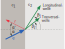
\includegraphics[scale=1.5]{oblique_angle_of_incidence}
	\caption{Representation of a sound wave $e$ shown in blue that hits an interface between the two media $Z_1$ and $Z_2$ with an oblique angle of incidence. The reflected wave $r$ is shown in red and the refracted transverse and longitudinal waves are shown in green \cite{ultrasound}.}
	\label{fig:oblique_angle_of_incidence}
\end{figure}

To calculate the angle of reflection shown in equation \ref{eq:oblique_angle_of_incidence} and the refraction shown in equation \ref{eq:oblique_refraction}, the same known laws from optics apply. Equation \ref{eq:oblique_refraction} allows the use of the transversal or longitudinal sound velocity for the variable $c_2$ depending on the desired result \cite{ultrasound}.

\begin{equation}
\alpha = \alpha^\prime
\label{eq:oblique_angle_of_incidence}
\end{equation}
\begin{equation}
\dfrac{\sin{(\alpha)}}{\sin{(\beta)}} = \dfrac{c_1}{c_2}
\label{eq:oblique_refraction}
\end{equation}
where:
\begin{multicols}{2}
\begin{conditions}
	\alpha & angle of incidence \\
	\beta & angle of refraction
\end{conditions}
\begin{conditions}
	\alpha^\prime & angle of reflection \\
	c_1 \text{, } c_2 & sound velocity in the medium
\end{conditions}
\end{multicols}


%-------------------------------------------------------------------------------------------
\subsection{Total Internal Reflection}
\label{subsec:Total_Internal_Reflection}
Total internal reflection can take place at the interface between two media. This happens when the following equation is valid:

\[
\sin{(\alpha_\text{crit})} = \dfrac{c_1}{c_2}
\]

This is a variation of the above shown equation \ref{eq:oblique_refraction}. Thus, the angle of refraction $\beta$ has to be 90\textdegree\ for the equation to be valid. For $\alpha \geq \alpha_\text{crit}$ the wave is totally reflected \cite{ultrasound}.

%-------------------------------------------------------------------------------------------
\subsection{Absorption}
\label{subsec:Absorption}
Sound waves are attenuated when they propagate in a medium due to absorption and scattering. Absorption usually converts a part of the ultrasound wave into heat. Scattering leads a particle that has been excited by the incoming wave to emit a wave in all direction itself. Equation \ref{eq:absorption} shows the exponential attenuation for monochromatic radiation. The \textbf{higher the frequency}, the \textbf{stronger the absorption} and scattering \cite{ultrasound}.

\begin{equation}
\hat{p}(x) = \hat{p}_0 \cdot e^{-\mu x}
\label{eq:absorption}
\end{equation}
where:
\begin{multicols}{2}
\begin{conditions}
	\hat{p}(x) & attenuated amplitude \\
	\mu & attenuation coefficient in m$^{-1}$
\end{conditions}
\begin{conditions}
	\hat{p}_0 & initial amplitude \\
	x & distance in m
\end{conditions}
\end{multicols}

%-------------------------------------------------------------------------------------------
\subsection{Ultrasound Generation}
\label{subsec:Ultrasound_Generation}
Ultrasound can be generated and received by using a ultrasonic transducer. In this experiment the piezoelectric effect is used in the ultrasonic transducer. Certain crystals expand proportional to the applied voltage. Contrary to this, the piezoelectric transducer induces a voltage when deformed. Thus, it can be used as a transmitter or receiver \cite{ultrasound}.

\begin{figure}[H]
	\centering
	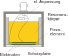
\includegraphics[scale=1.5]{ultrasound_generation}
	\caption{Graphical representation of a piezoelectric transducer. The active part is the thin piezo disk at the bottom of the transducer. The mechanical dimensions determine the resonance frequency of the oscillation. The transducer is impedance matched to the amplifier \cite{ultrasound}.}
	\label{fig:ultrasound_generation}
\end{figure}

\newpage
%-------------------------------------------------------------------------------------------
\subsection{Ultrasound Measurement}
\label{subsec:Ultrasound_Measurement}
There are two common ways to measure ultrasound, the A-Scan and the B-Scan. This experiment uses the A-Scan as measurement method and therefore only this one will be explained.

The A-Scan is a one-dimensional procedure where short ultrasound impulses ($f > 20 \text{kHz}$) are transmitted. These are partially reflected on the interfaces between media and are received again by the transmitter. From the time difference between the sent impulse and the received echo and a known distance, the sound velocity of a medium can be determined. Equation \ref{eq:sound_velocity} shows this relationship \cite{ultrasound}.

\begin{equation}
c_m = \dfrac{2x}{\Delta t}
\label{eq:sound_velocity}
\end{equation}
where:
\begin{multicols}{2}
	\begin{conditions}
		c_m & sound velocity of a medium in $\,^{\text{m}}\!/_{\text{s}}$ \\
		\Delta t & time difference in s
	\end{conditions}
	\begin{conditions}
		x & distance to interface in m
	\end{conditions}
\end{multicols}

This technique is often used to check the integrity of materials. If the part has defects such as cracks or inclusions of different substances, there are detectable echoes. Furthermore, the wall thickness of work pieces can be determined by this method \cite{ultrasound}.
